\begin{center}
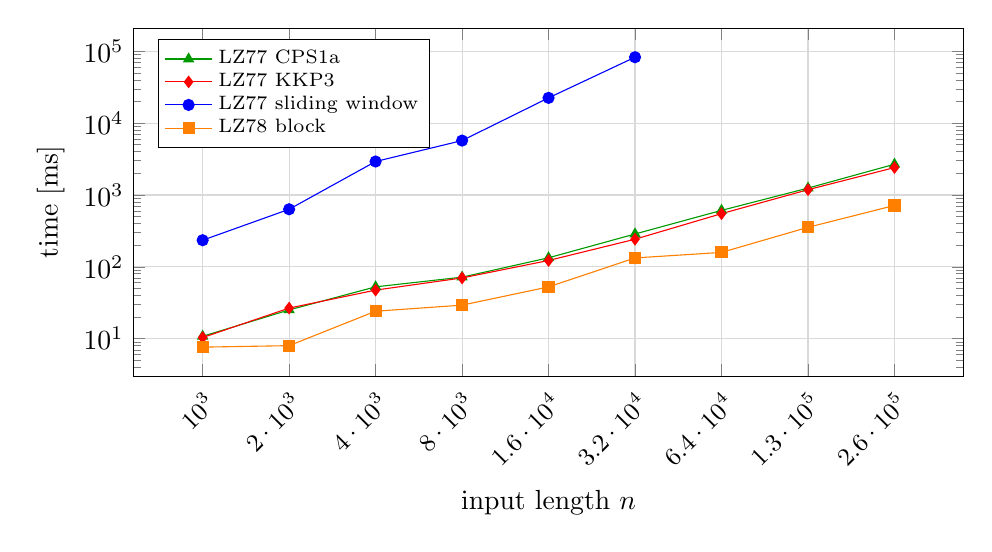
\begin{tikzpicture}
\begin{axis}[
  width = \linewidth, height = 6cm,
  xlabel = {input length $n$}, ylabel = {time [ms]},
  xmode = log, ymode = log,
  legend pos = north west, legend cell align = left,
  legend style = {font = \scriptsize, row sep = -2pt, inner sep = 2pt},
  xmajorgrids = true, ymajorgrids = true,
  xminorgrids = false, yminorgrids = false,
  minor tick num = 0,
  grid style = {draw = gray!30},
  xtick = {1000, 2000, 4000, 8000, 16000, 32000, 64000, 128000, 256000},
  xticklabels = {$10^{3}$, $2 \cdot 10^{3}$, $4 \cdot 10^{3}$, $8 \cdot 10^{3}$, $1.6 \cdot 10^{4}$, $3.2 \cdot 10^{4}$, $6.4 \cdot 10^{4}$, $1.3 \cdot 10^{5}$, $2.6 \cdot 10^{5}$},
  x tick label style = {rotate = 45, anchor = north east, font = \small},
]
\addplot[color = green!60!black, mark = triangle*] coordinates {(1000, 10.79) (2000, 25.11) (4000, 52.62) (8000, 71.76) (16000, 133.5) (32000, 286.24) (64000, 610.1) (128000, 1246.03) (256000, 2676.51)};
\addlegendentry{LZ77 CPS1a}
\addplot[color = red, mark = diamond*] coordinates {(1000, 10.36) (2000, 26.63) (4000, 47.39) (8000, 70.0) (16000, 122.47) (32000, 241.99) (64000, 549.13) (128000, 1183.11) (256000, 2405.25)};
\addlegendentry{LZ77 KKP3}
\addplot[color = blue, mark = *] coordinates {(1000, 234.39) (2000, 632.04) (4000, 2921.45) (8000, 5712.69) (16000, 22457.89) (32000, 82635.17)};
\addlegendentry{LZ77 sliding window}
\addplot[color = orange, mark = square*] coordinates {(1000, 7.62) (2000, 7.99) (4000, 24.09) (8000, 29.27) (16000, 52.51) (32000, 132.83) (64000, 158.65) (128000, 354.64) (256000, 714.29)};
\addlegendentry{LZ78 block}
\end{axis}
\end{tikzpicture}
\captionof{figure}{random 26, encoding time.}
\label{fig:random-26-encoding}
\end{center}

\begin{center}
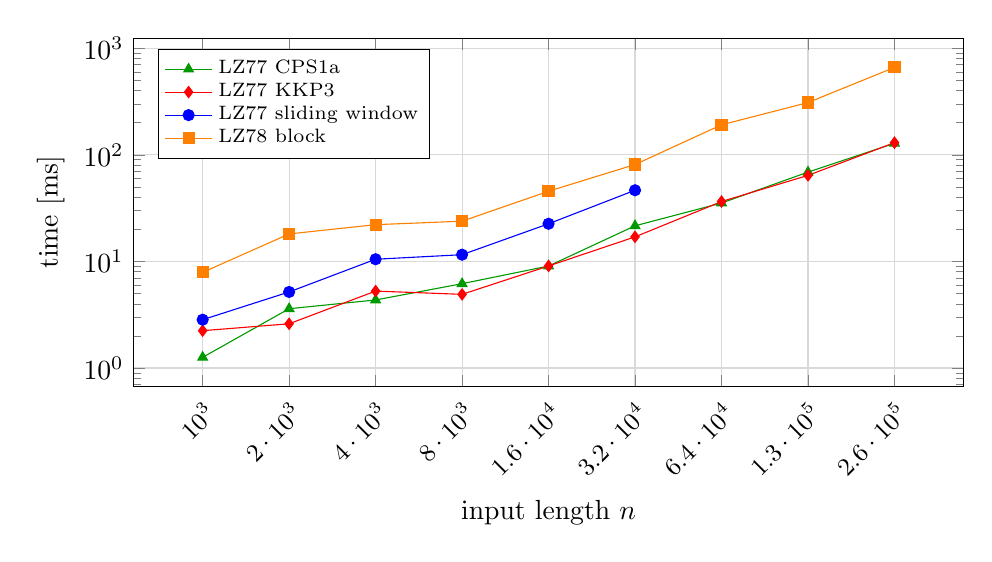
\begin{tikzpicture}
\begin{axis}[
  width = \linewidth, height = 6cm,
  xlabel = {input length $n$}, ylabel = {time [ms]},
  xmode = log, ymode = log,
  legend pos = north west, legend cell align = left,
  legend style = {font = \scriptsize, row sep = -2pt, inner sep = 2pt},
  xmajorgrids = true, ymajorgrids = true,
  xminorgrids = false, yminorgrids = false,
  minor tick num = 0,
  grid style = {draw = gray!30},
  xtick = {1000, 2000, 4000, 8000, 16000, 32000, 64000, 128000, 256000},
  xticklabels = {$10^{3}$, $2 \cdot 10^{3}$, $4 \cdot 10^{3}$, $8 \cdot 10^{3}$, $1.6 \cdot 10^{4}$, $3.2 \cdot 10^{4}$, $6.4 \cdot 10^{4}$, $1.3 \cdot 10^{5}$, $2.6 \cdot 10^{5}$},
  x tick label style = {rotate = 45, anchor = north east, font = \small},
]
\addplot[color = green!60!black, mark = triangle*] coordinates {(1000, 1.26) (2000, 3.6) (4000, 4.35) (8000, 6.18) (16000, 9.05) (32000, 21.57) (64000, 35.27) (128000, 68.81) (256000, 128.13)};
\addlegendentry{LZ77 CPS1a}
\addplot[color = red, mark = diamond*] coordinates {(1000, 2.24) (2000, 2.6) (4000, 5.27) (8000, 4.91) (16000, 9.06) (32000, 16.99) (64000, 36.43) (128000, 64.13) (256000, 129.82)};
\addlegendentry{LZ77 KKP3}
\addplot[color = blue, mark = *] coordinates {(1000, 2.84) (2000, 5.17) (4000, 10.48) (8000, 11.56) (16000, 22.54) (32000, 46.49)};
\addlegendentry{LZ77 sliding window}
\addplot[color = orange, mark = square*] coordinates {(1000, 7.89) (2000, 18.1) (4000, 22.11) (8000, 23.83) (16000, 45.53) (32000, 81.01) (64000, 191.03) (128000, 308.84) (256000, 659.92)};
\addlegendentry{LZ78 block}
\end{axis}
\end{tikzpicture}
\captionof{figure}{random 26, decoding time.}
\label{fig:random-26-decoding}
\end{center}

\begin{center}
\begin{tabular}{lrrrrrr}
\hline
algorithm & $n$ & $\alpha$ & $z$ & $\rho$ & encode [ms] & decode [ms] \\
\hline
LZ77 sliding window & 32000 & 26 & 9083 & 2.5546 & 81989.29 & 51.75 \\
LZ78 block & 32000 & 26 & 10192 & 1.1534 & 78.4 & 131.06 \\
LZ77 CPS1a & 32000 & 26 & 9083 & 1.7031 & 343.46 & 24.88 \\
LZ77 KKP3 & 32000 & 26 & 9083 & 1.7031 & 297.18 & 17.13 \\
\hline
\end{tabular}
\captionof{table}{random 26: uniform over the lowercase latin alphabet.}
\label{tab:random-26}
\end{center}